%
% To make graphic on linux....(require ImageMagic installed)
%
% pdflatex thisfile.tex
% convert -density 300 thisfile.pdf -resize 640x480 thatfile.png 
%
% On Windows 10.... copy ImageMagic's convert.exe to your path 
% or rename it imgconvert.exe
% Get recent version of GhostScript
%
% pdflatex thisfile.tex
% convert -density 300 thisfile.pdf -resize 640x480 thatfile.png 
%
% Trouble? See this thread
%
% https://tex.stackexchange.com/questions/11866/compile-a-latex-document-into-a-png-image-thats-as-short-as-possible/11880#11880
%
\documentclass{standalone}
\usepackage{tikz}

\author{CC-BY-2016 James B. Wilson}
\date{2016}
\date{today}
\begin{document}
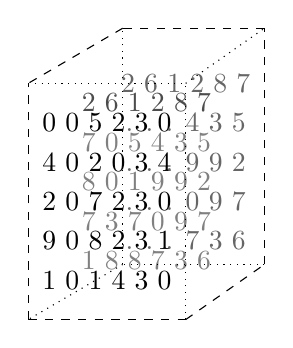
\begin{tikzpicture}
	\coordinate (A1) at (.5,0);
	\coordinate (A2) at (2.5,0);
	\coordinate (A3) at (3.5,0.7);
	\coordinate (A4) at (1.7,0.7);
	\coordinate (A5) at (.5,3);
	\coordinate (A6) at (2.5,3);
	\coordinate (A7) at (3.5,3.7);
	\coordinate (A8) at (1.7,3.7);
	\node at (1.5,0.5) {1 0 1 4 3 0}; 
	\node at (1.5,1.0) {9 0 8 2 3 1}; 
	\node at (1.5,1.5) {2 0 7 2 3 0}; 
	\node at (1.5,2.0) {4 0 2 0 3 4}; 
	\node at (1.5,2.5) {0 0 5 2 3 0}; 
	
	\node[color=gray] at (2,0.75) {1 8 8 7 3 6}; 
	\node[color=gray] at (2,1.25) {7 3 7 0 9 7}; 
	\node[color=gray] at (2,1.75) {8 0 1 9 9 2}; 
	\node[color=gray] at (2,2.25) {7 0 5 4 3 5}; 
	\node[color=black!70] at (2,2.75) {2 6 1 2 8 7}; 
	
	\node[color=black!60] at (2.5,1.0) {.  .  .  7 3 6}; 
	\node[color=black!60] at (2.5,1.5) {.  .  .  0 9 7}; 
	\node[color=black!60] at (2.5,2.0) {.  .  .  9 9 2}; 
	\node[color=black!60] at (2.5,2.5) {.  .  .  4 3 5}; 
	\node[color=black!60] at (2.5,3.0) {2 6 1 2 8 7}; 
	
	\draw[dashed] (A1) -- (A2);
	\draw[dashed] (A2) -- (A3);
	\draw[dotted] (A3) -- (A4);
	\draw[dotted] (A4) -- (A1);
	\draw[dotted] (A4) -- (A8);
	\draw[dashed] (A1) -- (A5);
	\draw[dotted] (A5) -- (A6);
	\draw[dotted] (A6) -- (A7);
	\draw[dashed] (A7) -- (A8);
	\draw[dashed] (A8) -- (A5);
	\draw[dotted] (A2) -- (A6);
	\draw[dashed] (A3) -- (A7);
\end{tikzpicture}
\end{document}
